\chapter{Des atomes de Rydberg froids en environnement cryogénique}
\label{chapter:setup_coldatoms_Rydberg}

INTRODUCTION DU CHAPITRE\\
entre autres, longue vie aux Rydberg en environnement cryogénique\\
renvoi aux thèses précédentes pour plus de détail (Raul, T. Nirrengarten, C. Roux)

\section{Un nuage d'atomes froids sur puce, du MOT de capture au condensat de Bose-Einstein}

OUAH COMMENT C4EST CHOUETTE LES ATOMES FROIDS

	\subsection{L'environnement cryogénique : cryostat et puce à atomes supraconductrice}\label{subsec:cryopuce}
	
\noindent L'environnement cryogénique présente un avantage incomparable pour la durée de vie des atomes de Rydberg, mais impose aussi quelques spécificités à notre dispositif d'atomes froids.
Le piégeage d'atomes froids pendant des durées suffisantes à leur manipulation exige un vide très poussé dans l'enceinte expérimentale, car les collisions avec les molécules de gaz résiduel éjectent les atomes hors de leur piège.
Les chambres de piégeage d'atomes neutres à température ambiante sont généralement étuvées pendant plusieurs semaines afin d'atteindre des pressions de gaz résiduel suffisamment faibles.
Dans un environnement cryogénique au contraire, les parois froides de l'enceinte adsorbent une grande partie du gaz résiduel, et des pressions inférieures à \SIvv{1e-10}{\milli\bar} sont obtenues sans étuvage.
Travailler en environnement cryogénique permet en outre l'utilisation de fils et de bobines supraconducteurs pour le passage des courants électriques qui génèrent les champs magnétiques nécessaires au piégeage des atomes.
Des courants de quelques Ampères sont ainsi passés sans dissipation et à proximité des atomes piégés, alors qu'une expérience d'atomes froids à température ambiante nécessite des bobines qui soient placées en-dehors de la chambre et refroidies par des circuits dédiés.

L'environnement cryogénique pour les atomes froids a cependant quelques inconvénients :
en premier lieu, l'accès optique est limité car les parois de l'enceinte doivent être opaques pour le rayonnement du corps noir et donc métalliques, chaque hublot de verre réduisant l'isolation thermique du c\oe ur de l'expérience.
En second lieu, l'utilisation d'hélium et d'azote liquide au contact d'un vide poussé présente une lourdeur technique supplémentaire au quotidien.

	\subsubsection*{Le cryostat}
\noindent Notre expérience est placée au c\oe ur du cryostat représenté en figure \eqref{fig:cryo}.
%
\begin{figure}
\centering
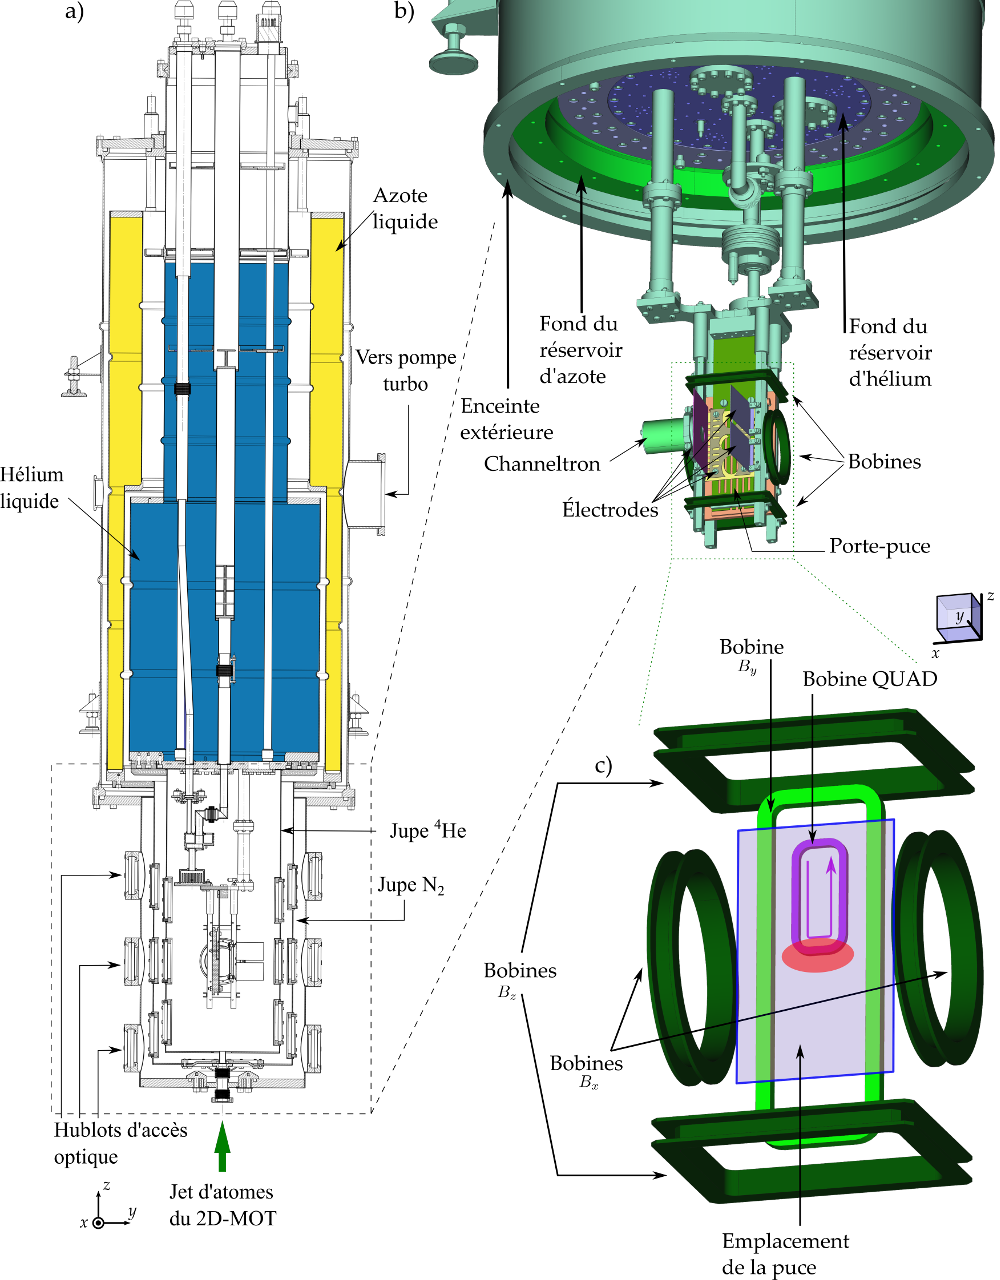
\includegraphics[width=\linewidth]{figures/cryo_vect_small.png}
\caption[Schéma du cryostat]{Schéma du dispositif cryogénique :
\textbf{a)} coupe du plan de construction du cryostat, avec la puce tournée vers le côté gauche.
Le réservoir d'azote liquide est indiqué en jaune, le réservoir d'hélium liquide en bleu.
Le c\oe ur de l'expérience est visible, ainsi que les deux \og jupes \fg{} et l'enceinte extérieure à température ambiante.
Cinq hublots, trois en face de la puce et un sur chaque côté, sont installés sur chacune de ces jupes pour l'accès optiques.
\textbf{b)} vue schématique du c\oe ur de l'expérience. La puce fait face à la direction $y$. Les bobines (vert foncé), le channeltron et les différentes électrodes sont représentées. On ne voit pas les \og jupes \fg{} d'azote et d'hélium, ni l'enceinte extérieure.
\textbf{c)} Vue de plus près des bobines : la bobine QUAD (mauve) génère un champ quadrupolaire pour faire un MOT sur puce. L'emplacement de la puce est représenté par le rectangle bleu devant la bobine QUAD et la bobine $B_y$ (vert clair).
La zone rouge indique l'endroit où les atomes de rubidium sont piégés.
}
\label{fig:cryo}
\end{figure}
%
La conception de ce cryostat a été évoquée dans la thèse de Raul Celistrino Teixeira \cite{PHD_CELISTRINO}  et discutée plus en détail dans les thèses de Thomas Nirrengarten \cite{PHD_NIRRENGARTEN} et Cédric Roux \cite{PHD_ROUX}.
Le c\oe ur de l'expérience est protégé de la radiation extérieure par des écrans thermiques (\og jupes \fg{}) en cuivre doré. Ce sont des cylindre ouverts en haut et vissés sur le fond des réservoirs de liquides cryogéniques.
La jupe $^4 \text{He}$ est vissée sur le fond du réservoir d'hélium 4 et la jupe $\text{N}_2$ est vissée au fond du réservoir d'azote liquide.
Elles sont donc respectivement thermalisées à \SIvv{4.2}{\K} et \SIvv{77}{\K}.
Sur chaque jupe, cinq hublots sont installés pour l'accès optique à la zone de piégeage :
deux sur les directions $\pm x$, un dans la direction $+y$ qui fait face à la puce, et deux  sur le plan $yz$, de part et d'autre du hublot de face sur les bissectrices des axes $+y$ et $\pm z$, appelées direction $\pm\SIvv{45}{\degree}$ respectivement.
Par ces hublots, tous les faisceaux laser atteignent la zone de piégeage au c\oe ur de l'expérience.
Tous les éléments qui sont installés à l'intérieur de la jupe hélium sont thermalisés à \SIvv{4.2}{K} par contact thermique avec le réservoir d'hélium liquide.

L'intérieur de la jupe hélium est revêtu d'une couche de plomb, supraconducteur à \Khe. Cette couche de plomb écrante les champs magnétiques extérieurs par effet Meissner \cite{MX_MEISSNEREFFECT}, et évite les courants de Foucault qui se créeraient dans les jupes à l'allumage ou à l'extinction des courants dans les bobines. 
Il reste nécessaire cependant d'imposer un champ extérieur de compensation au moment du refroidissement, afin que la couche de plomb ne piège pas de lignes de champ magnétique provenant de l'environnement.
Cette compensation du champ constant de l'environnement est réalisée à l'aide de grandes bobines placées à l'extérieur du crysotat.

Enfin, bien que les jupes ne soient pas parfaitement étanches, elles garantissent un vide différentiel entre la partie du cryostat à \SIvv{300}{\K}, où la pression vaut \SIvv{1.5e-7}{\milli\bar}, et la partie à \Khe, où la pression est inférieure à \SIvv{1e-10}{\milli\bar}\footnote{
Cette valeur n'est pas mesurée en raison de l'absence de sonde de pression dans cette région du cryostat, mais inférée à partir du temps de vie des nuages d'atomes piégés, qui est de l'ordre de la minute \cite{ENS_CHIPLIFETIME}.}.

	\subsubsection*{La puce à atomes}
\noindent La puce à atome qui siège au c\oe ur de notre expérience est représentée en figure \eqref{fig:chip}.
C'est une puce assez simple, conçue autour de trois fils supraconducteurs : le fil (LJ), en forme de \mcal{U}, le fil (LG) en forme de \mcal{Z}, et le fil (KM) droit.
Ces fils sont fabriqués par dépôt de niobium d'une épaisseur de \SIvv{2}{\um} sur un substrat de silicium recouvert d'une couche d'oxyde SiO$_2$.
Le dépôt de niobium est ensuite gravé, et l'ensemble de la puce est recouvert d'une couche d'or de \SIvv{200}{\nm} d'épaisseur afin de rendre la surface réfléchissante.
Les détails de la fabrication de la puce sont présentés en annexe dans la thèse de Raul Celistrino Teixeira \cite{PHD_CELISTRINO}.
%
\begin{figure}[]
\centering
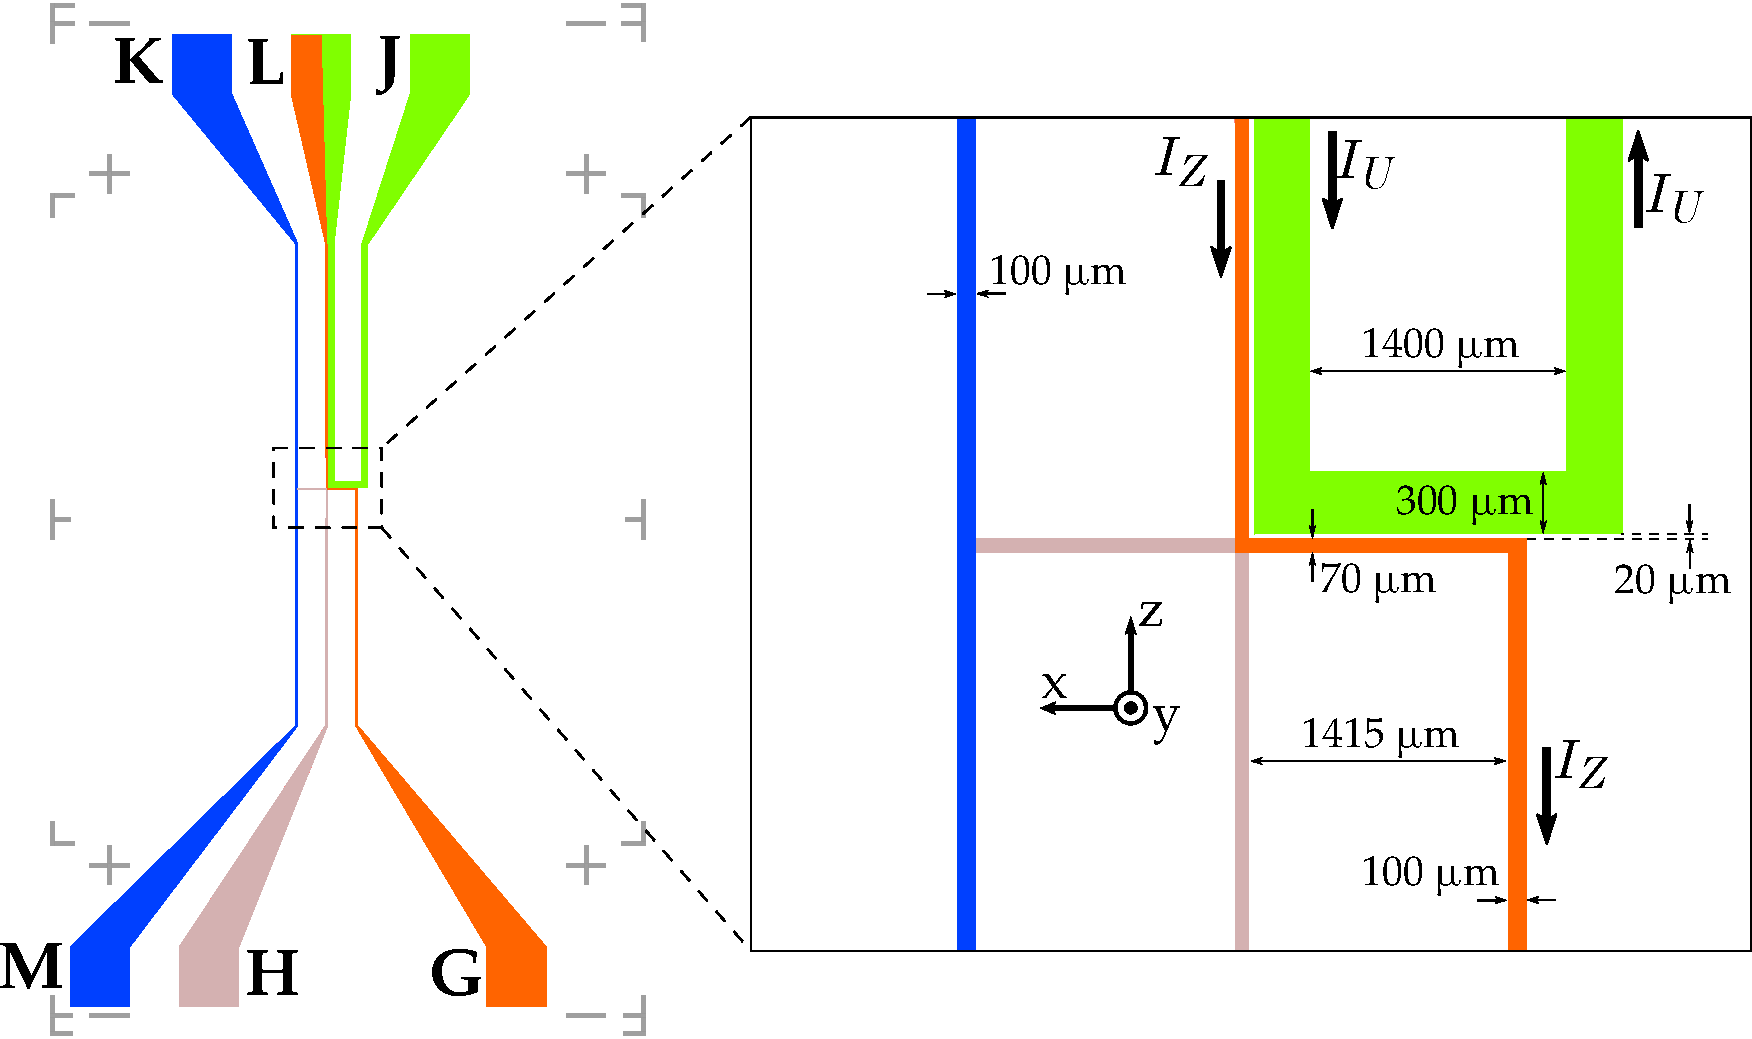
\includegraphics[width=\linewidth]{figures/chip}
\caption[Schéma de la puce à atomes supraconductrice]{Schéma de la puce supraconductrice.
Les lettres étiquettent les pattes d'entrée/sortie des courants électriques sur la puce.
Les couleurs sont une aide visuelle pour mieux suivre les fils : en vert, le \og fil \mcal{U}\fg{}, en orange le \og fil \mcal{Z}\fg{} et en bleu le \og fil RF \fg{}.
\`A droite, vue de près du centre de la puce, qui détaille la largeur des fils, la distance entre eux et le sens de circulation des courants.
Les axes $x,y$ et $z$ coïncident avec ceux de la figure \eqref{fig:cryo}.
}
\label{fig:chip}
\end{figure}
%

Les fils en \mcal{U} et en \mcal{Z} sont la simplification d'un dispositif en forme de $\mathcal{H}$ qui repose sur la circulation d'un courant perpendiculairement à deux autres courants parallèles entre eux.
La figure \eqref{fig:magfields_chip} représente les différentes configurations de champ magnétique créées par les fils \mcal{U} et \mcal{Z} de la puce.
Lors du passage d'un courant $I$ dans le fil \mcal{Z}, le segment parallèle à l'axe $x$ créé un champ qui, superposé avec un champ de biais $B_Z$ selon l'axe $z$, forme un champ quadrupolaire dans le plan $yz$.
Le courant dans les deux bras verticaux circule dans le même sens et crée un champ selon $x$, avec un  minimum non-nul au voisinage du centre du champ quadrupolaire.
Le champ total forme alors un piège magnétique de Ioffe-Pritchard (cf figure \ref{fig:magfields_chip}c)).

De façon similaire, le fil en \mcal{U} crée aussi, avec l'aide d'un champ de biais $B_Z$, un champ quadrupolaire dans le plan $yz$.
Les courants dans les bras verticaux circulent cette fois dans des sens opposés, ce qui résulte dans la présence d'un zéro de champ près du centre du champ quadrupolaire.
Le champ total permet ici la réalisation d'un piège magnéto optique sur puce en trois dimensions (\og 3D-MOT miroir\fg{}, cf figure \ref{fig:magfields_chip}d)).

\begin{figure}[]
\centering
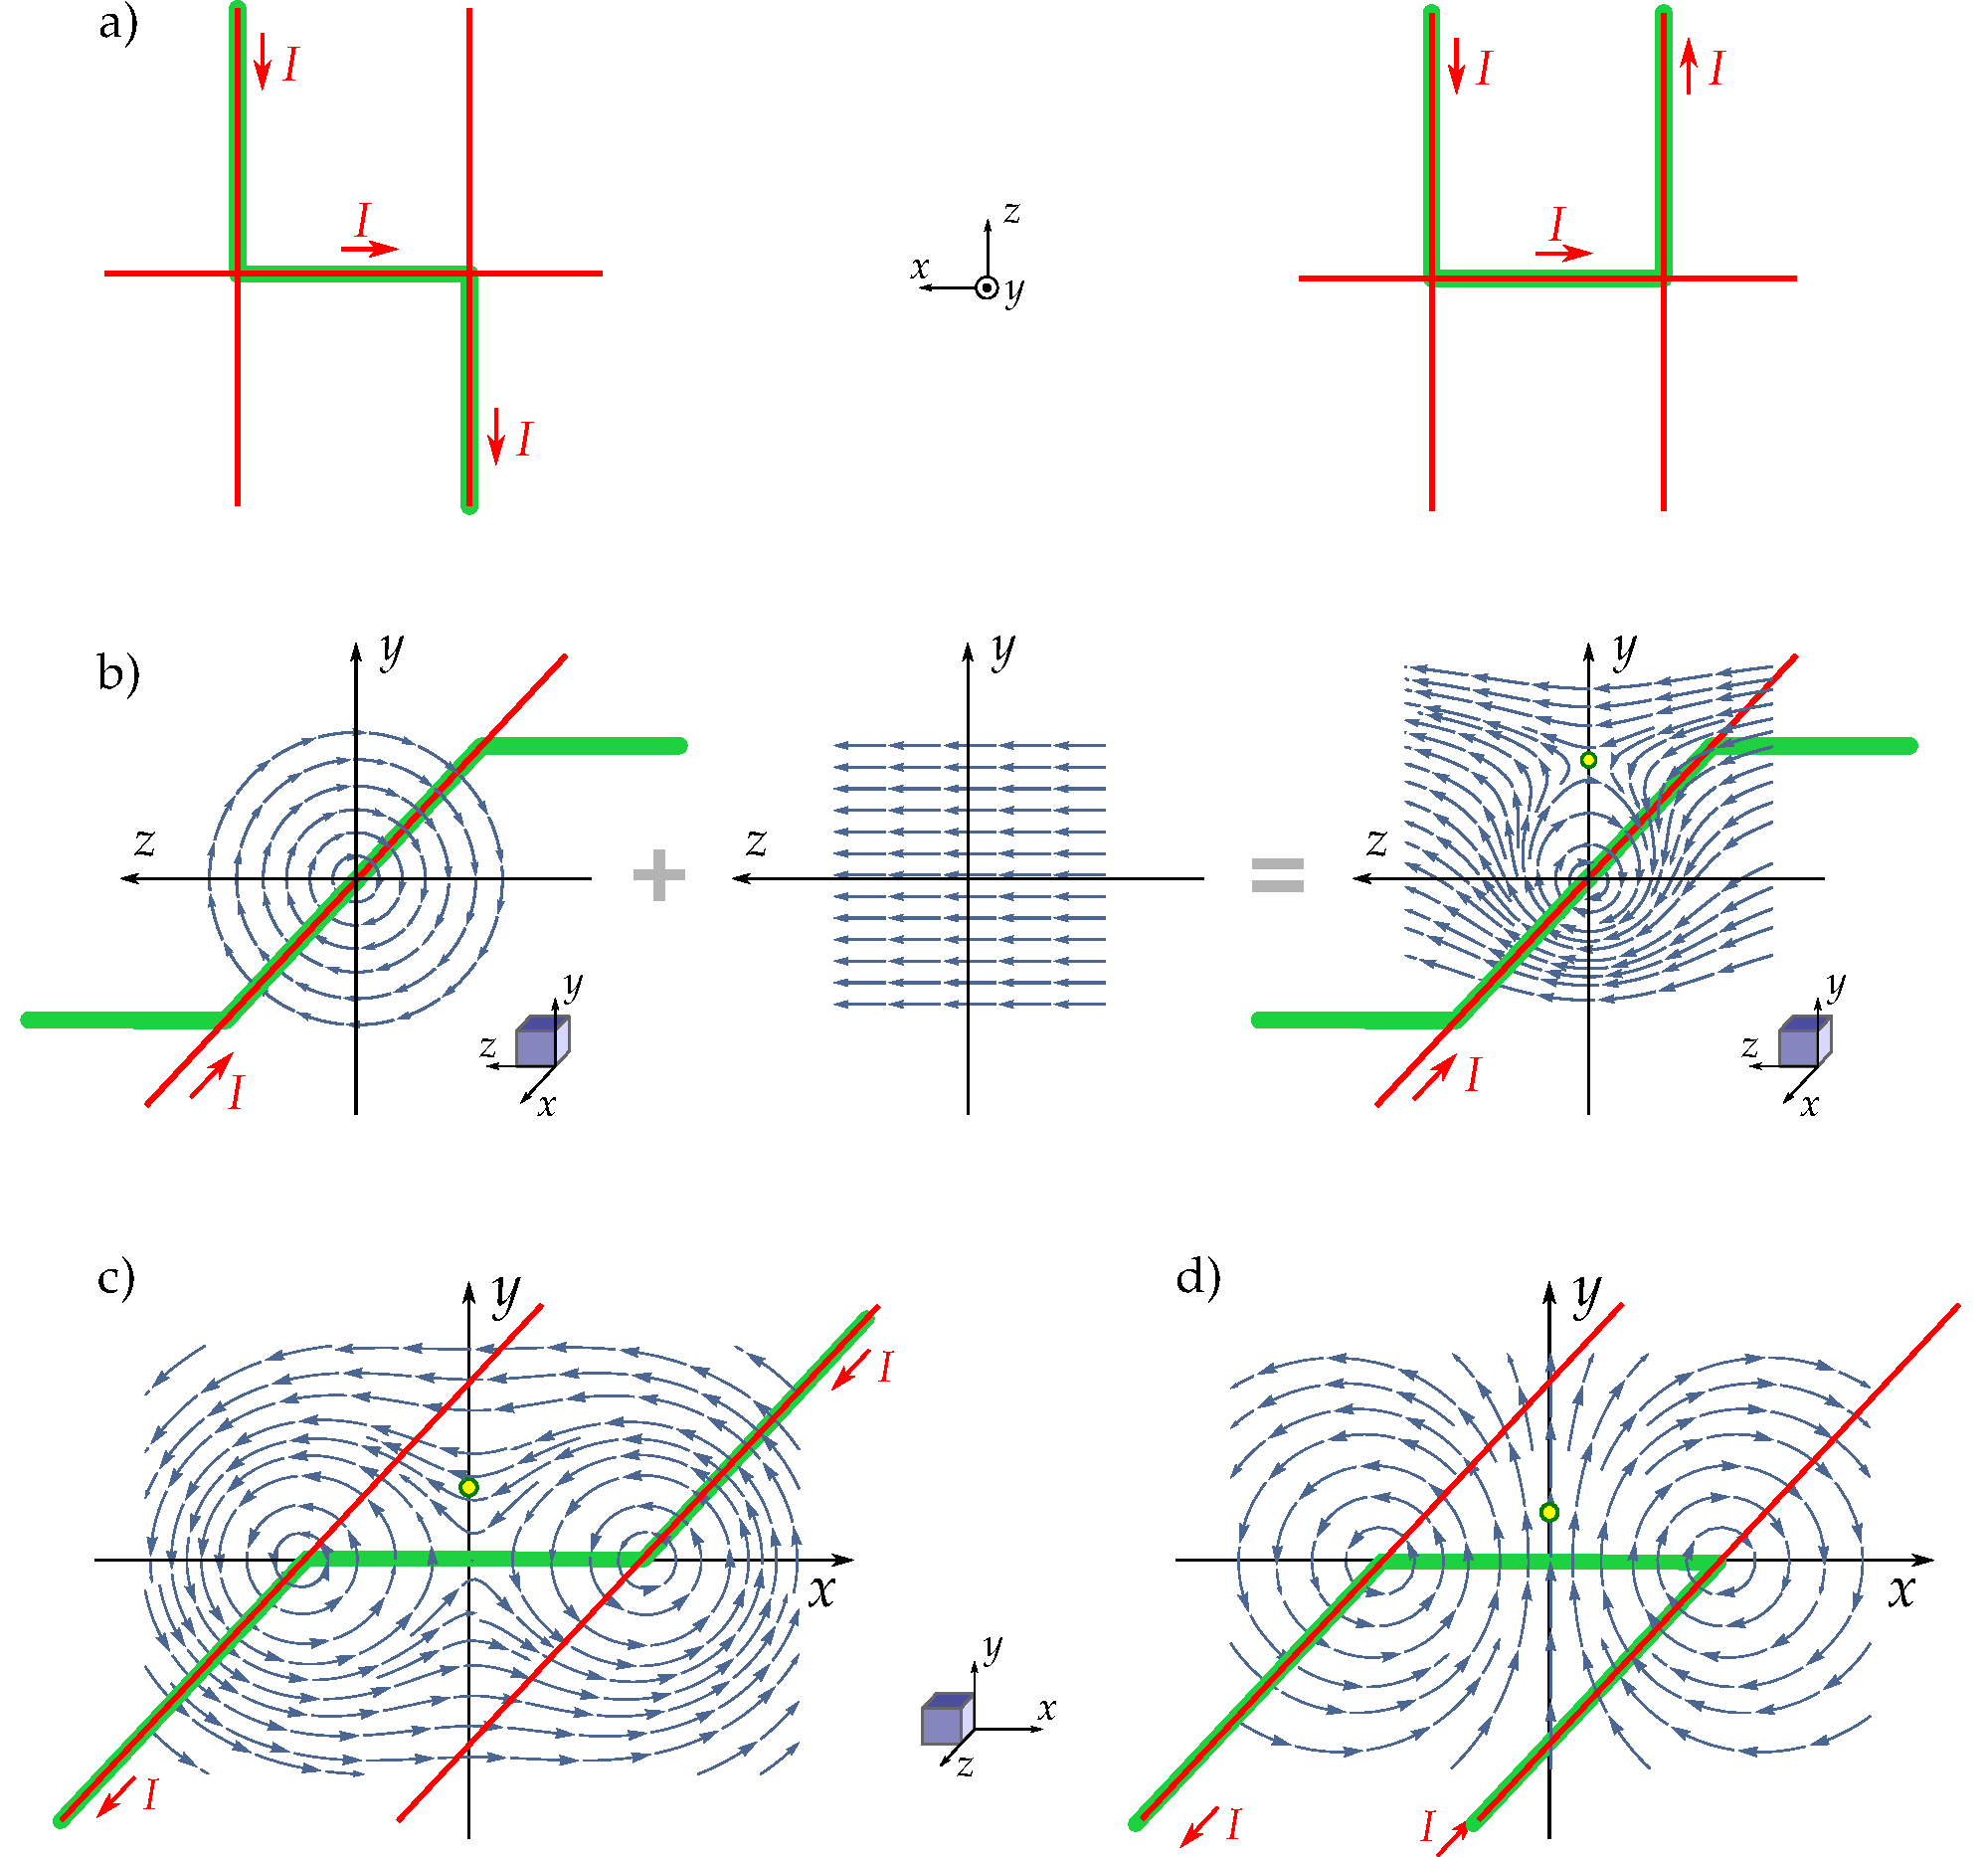
\includegraphics[width=\linewidth]{figures/magfields_chip}
\caption[Champs magnétiques créés par la puce]{
Champs magnétiques créés par la puce.
\textbf{a)} Les fils \mcal{U} et \mcal{Z} portent un courant dans la direction $x$ et une paire de courants parallèles dans la direction $z$.
\textbf{b)} Un champ quadrupolaire est créé par la superposition du courant selon $x$ et d'un champ de biais $B_Z$.
Les courants verticaux peuvent circuler soit (\textbf{c)}) dans le même sens,  soit (\textbf{d)}) dans des sens opposés.
Le module du champ total présentera alors respectivement un minimum non-nul ou nul aux positions marquées par les points jaunes.
}
\label{fig:magfields_chip}
\end{figure}

Pour le fil en \mcal{Z} comme pour le fil en \mcal{U}, le centre du piège se situe à une distance de la puce valant approximativement
\begin{equation}
\label{eq:trap_center}
r_0 \simeq \frac{\mu _0}{2\pi}\frac{I}{B_Z}
\end{equation}
et le gradient de champ magnétique à cet endroit vaut
\begin{equation}
\label{eq:trap_center_grad}
|B'(r_0)|=\frac{2\pi}{\mu _0} \frac{B_Z^2}{I} = \frac{B_Z}{r_0} = \frac{\mu _0}{2\pi}\frac{I}{r_0^2}~.
\end{equation}
%
C'est là une caractéristique importante de la géométrie des pièges : plus le centre du piège est proche de la puce, plus le piège sera confinant dans le plan $yz$.
Le piège s'allonge alors dans la direction $x$, prenant une forme de cigare de plus en plus anisotrope.

Comme nous l'avons mentionné, notre dispositif nous permet de mettre en \oe uvre des pièges magnéto-optiques en trois dimensions.
Dans beaucoup d'expériences d'atomes froids, ceux-ci sont réalisés à l'aide de trois paires de faisceaux laser contra-propageants, une dans chaque direction de l'espace.
Il nous est impossible d'envisager cette configuration, puisque l'axe $y$ est rendu inaccessible par la présence de la puce.
L'on peut cependant, avec deux paires de faisceaux laser seulement, simuler une configuration à six faisceaux, en utilisant la surface réfléchissante de la puce.
Le schéma de cette configuration, appelée \og MOT miroir \fg{}, est donné en figure \eqref{fig:mirror_MOT}.

\begin{figure}
\centering
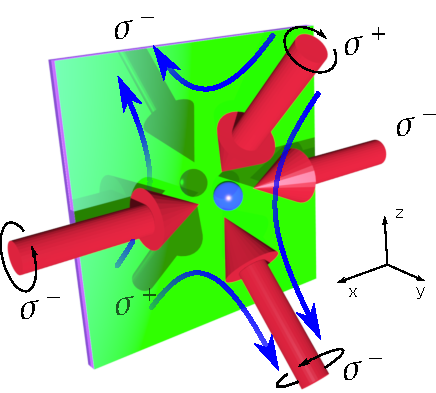
\includegraphics[width=0.6\linewidth]{figures/mirror_MOT}
\caption[Schéma de principe du MOT miroir]{Schéma de principe du MOT miroir :
Deux faisceaux contra-propageants sont envoyés parallèlement à la puce réfléchissante, selon l'axe $x$.
Les deux autres faisceaux dans le plan $yz$ viennent frapper la puce avec un angle de \SIvv{45}{\degree}.
Leur réflexion sur la puce équivaut à deux faisceaux supplémentaires d'hélicité inversée, représentés en ombre derrière la puce.
On obtient bien ainsi une configuration de MOT à six faisceaux.
}
\label{fig:mirror_MOT}
\end{figure}


	\subsection{Séquence de piégeage et refroidissement}
	
\noindent Grâce à ce dispositif, nous pouvons piéger des nuages d'atomes froids sur puce.
Nous donnons dans ce paragraphe le détail des différentes étapes de piégeage et de refroidissement des atomes.

	\subsubsection*{Système laser}
\noindent Le piégeage magnéto-optique du rubidium 87 exploite la raie D2 de celui-ci.
La raie D2 est représentée en figure \eqref{fig:D2lineRb87} avec le détail des sous-niveaux hyperfins des niveaux $\mathrm{5S_{1/2}}$ et $\mathrm{5P_{3/2}}$ du \Rb{87}.
%	
\begin{figure}
\centering
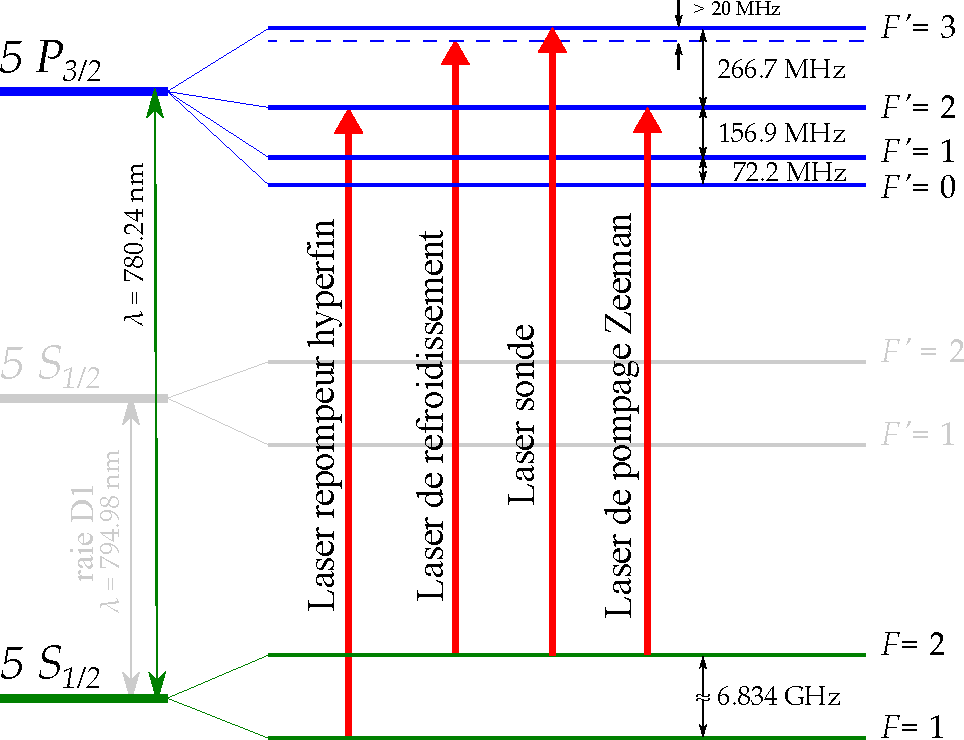
\includegraphics[width=0.8\linewidth]{figures/D2lineRb87}
\caption[Raie D2 du \Rb{87}]{Structure hyperfine de la raie D2 du \Rb{87}.
Les transitions cyclantes sont montrées pour le laser de refroidissement, le laser repompeur, le laser sonde et le laser de pompage Zeeman.
}
\label{fig:D2lineRb87}
\end{figure}
%
Nous utilisons la transition $\ket{F=2} \rightarrow \ket{F'=3}$ de la raie D2 pour piéger et refroidir les atomes.
Cette transition a une largeur naturelle $\Gamma = \SI{6.065}{\MHz}$ \cite{DATA_STECKRB87}.
Le laser de refroidissement est généré par un système commercial de diode laser amplifiée TOPTICA TA-110.
La fréquence de ce laser est asservie par battement (\og beatlock \fg{}) à un laser maître, lui-même stabilisé par une cavité Fabry-Pérot.
Cette cavité est verrouillée en fréquence sur la transition de refroidissement par absorption saturée dans une cellule de \Rb{87}.
Une commande de tension permet de définir la fréquence du battement et ainsi de contrôler rapidement le désaccord du laser de refroidissement par rapport à la transition $\ket{F=2}\rightarrow\ket{F'=3}$.

Il arrive qu'un photon du laser de refroidissement excite un atome du niveau $\ket{F=2}$ vers le niveau $\ket{F'=2}$ au lieu de $\ket{F'=3}$.
Cet atome peut alors se désexciter non pas vers le niveau $\ket{F=2}$ mais vers le niveau $\ket{F=1}$, qui est un niveau noir pour le laser de refroidissement.
Afin d'éviter le pompage des atomes vers ce niveau $\ket{F=1}$, il est nécessaire d'envoyer, avec le laser de refroidissement, un laser \og repompeur\fg{} accordé sur la transition $\ket{F=1}\rightarrow \ket{F'=2}$.
Ce laser repompeur est généré par une troisième diode laser, et indépendamment verrouillé en fréquence par absorption saturée.

Les lasers de sonde et de pompage Zeeman sont prélevés sur le laser de refroidissement et décalés en fréquence par modulation acousto-optique.
L'ensemble des faisceaux est transporté de la table optique de préparation au cryostat par des fibres optiques mono-modes à maintien de polarisation.
Ils sont enfin mis en forme à proximité immédiate du cryostat. 




	\subsubsection*{Piégeage magnéto-optique}
\noindent	Notre dispositif repose sur trois stades de piégeage magnéto-optique successifs.
Les atomes de rubidium sont stockées dans une cellule en verre, ouverte vers une enceinte sous ultra-vide (UHV) située à l'extérieur du cryostat.
Dans cette enceinte, les atomes sont piégés le long de l'axe $z$ par un piège magnéto-optique en deux dimensions (\og 2D-MOT \fg{}).
Celui-ci est schématisé en figure \eqref{fig:2DMOT}.
%	
\begin{figure}
\centering
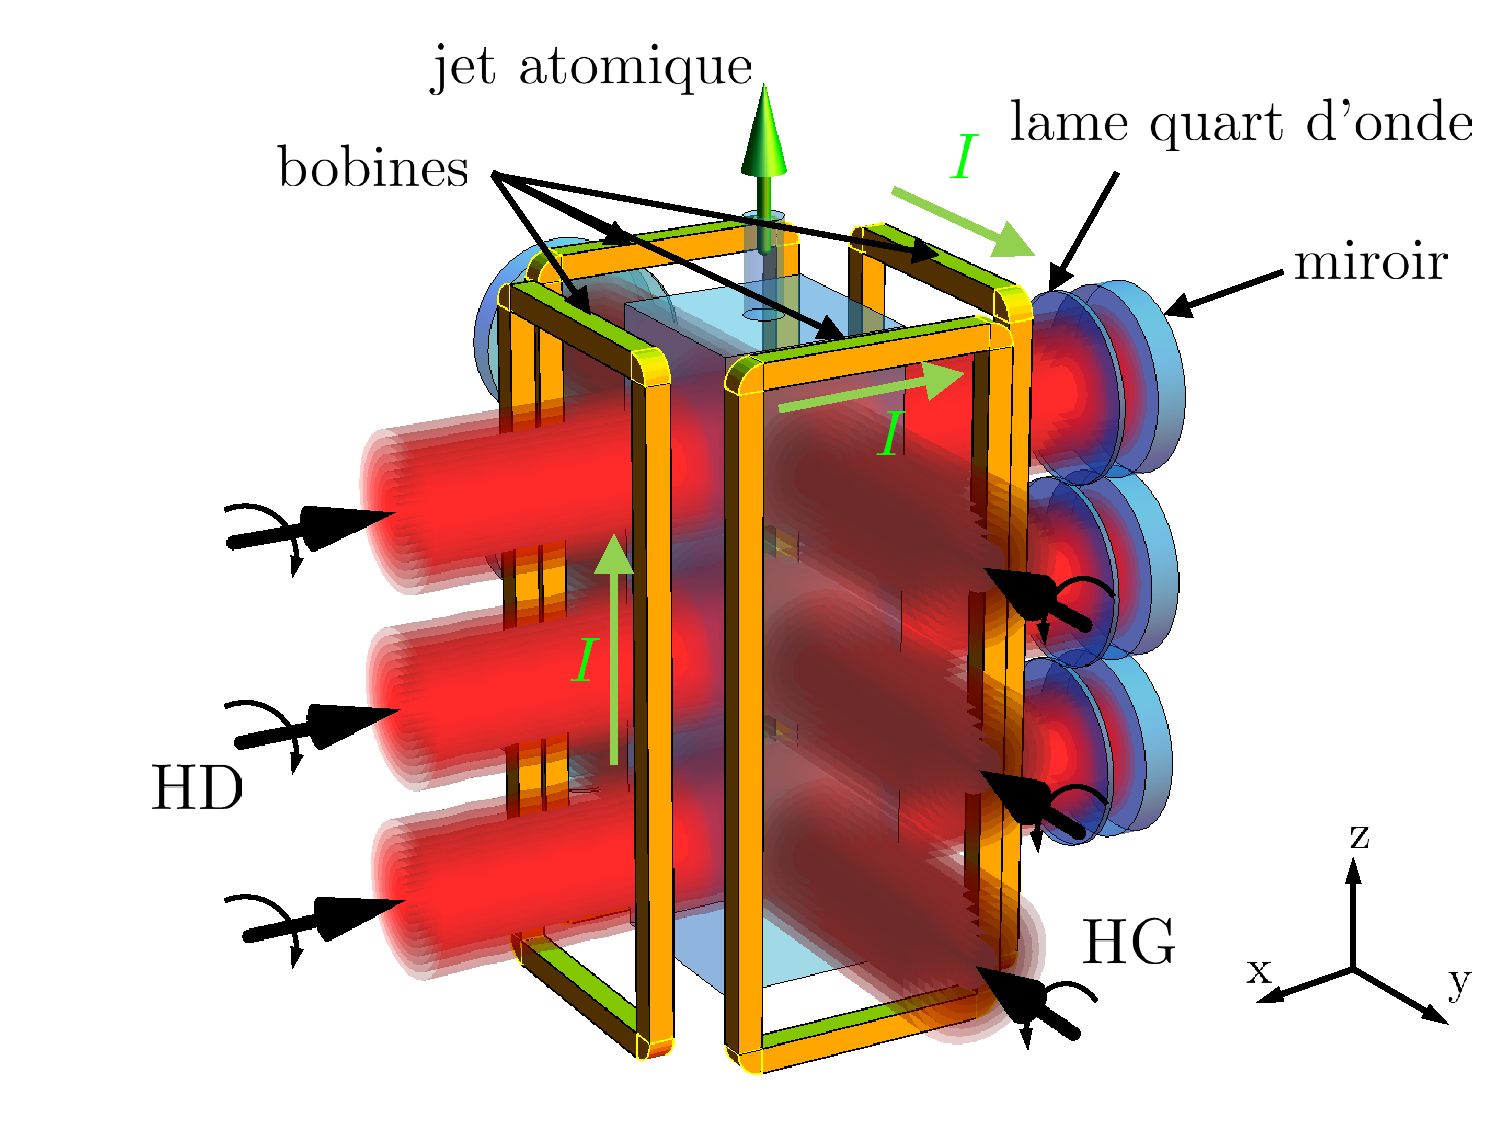
\includegraphics[width=0.6\linewidth]{figures/2DMOT}
\caption[Schéma du 2D-MOT]{Schéma du 2D-MOT avec ses trois étages de piégeage.
Les polarisations des faisceaux incidents sont indiquées par les lettres HD (pour hélicité droite) et HG (hélicité gauche), relativement à la direction de propagation des faisceaux.
Le sens des courants dans les bobines est indiqué par les flèches verts et la lettre $I$.
Chaque faisceau est rétro-réfléchi par un miroir, et le double passage par une lame quart d'onde permet de garantir la bonne polarisation du faisceau réfléchi.
Le jet atomique produit par le 2D-MOT est représenté par une flèche qui pointe vers le cryostat.
}
\label{fig:2DMOT}
\end{figure}
%
L'ensemble du 2D-MOT a été conçu et fabriqué par la laboratoire SYRTE de l'Observatoire de Paris.

Les atomes piégés dans le 2D-MOT diffusent librement selon l'axe $z$, formant un jet vertical qui arrive jusqu'à la puce atomique à l'intérieur du cryostat.
Les atomes sont alors capturés dans un MOT de grand volume créé par les bobines de biais et le bas de la bobine \og QUAD \fg{}, représentée en figure \eqref{fig:cryo}.
Le bas de la bobine QUAD permet de créer un champ quadrupolaire similaire à celui du fil \mcal{U}, adapté au piégeage magnéto-optique.
Le nombre de spires $n=19$ de la bobine permet de multiplier par autant le courant générateur de champ dans l'équation \eqref{eq:trap_center}.
Le grand volume du champ quadrupolaire ainsi créé permet de capturer efficacement les atomes du jet.
Le chargement de ce gros \og QAUD-MOT \fg{} dure de \SIvv{1}{} à \SIvv{3}{\s}, pendant lesquels on peut y collecter quelques \SIvv{e8} atomes à une température de l'ordre de \SIvv{400}{\uK}.

Le nuage atomique est alors transféré vers un second MOT, créé cette fois par les bobines de biais et le fil \mcal{U}, comme nous l'avons mentionné en \ref{subsec:cryopuce}.
Ce \og U-MOT lointain\fg{} présente des gradients similaires au QUAD-MOT mais un volume plus petit.
Le taux de transfert entre les deux est estimé entre $\num{10}$ et $\SI{40}{\percent}$ par des observations en fluorescence du nuage.
Nous pouvons à ce moment réduire le courant dans le fil \mcal{U}, ce qui d'après les équations \eqref{eq:trap_center} et \eqref{eq:trap_center_grad} rapproche le piège de la surface de la puce et le comprime en augmentant le gradient de champ.
Les gradients de champs étant plus forts, la force de rappel de la lumière s'en trouve grandie.
On peut alors se permettre d'augmenter le désaccord des faisceaux lasers afin de refroidir le nuage atomique.
Les températures atteintes dans ce \og U-MOT proche\fg{} sont de l'ordre de $\SI{40}{\uK}$, pour un nuage d'environ $\numrange{e7}{e8}$ atomes.

	\subsubsection*{Les étapes intermédiaires : mélasse optique et pompage Zeeman}
L'objectif, après les étapes de piégeage magnéto-optique, est de transférer les atomes dans le piège de Ioffe-Pritchard créé par le fil \mcal{Z}.
Cela sera d'autant plus efficace que le nuage atomique sera froid, et que les atomes seront bien polarisés dans le sous-niveau Zeeman $m_F=+2$ du niveau hyperfin $\mathrm{5S1/2,F=2}$.
Avant de les transférer vers le \og piège Z \fg{}, nous faisons donc subir aux atomes deux phases supplémentaires.

Tout d'abord, nous éteignons les champs magnétiques du U-MOT en laissant les faisceaux lasers allumés.
Cela initie une étape de mélasse optique d'une durée comprise entre $\num{1} et \SI{5}{\ms}$, au cours de laquelle le désaccord laser est augmenté alors que la puissance lumineuse est graduellement diminuée jusqu'à zéro.
Cette mélasse optique nous permet de refroidir quelques $\numrange{e6}{e7}$ atomes à des températures de l'ordre de $\SIvv{10}{\uK}$.

Après l'extinction des lasers de mélasse, un champ magnétique de \SIrange{1}{2}{\gauss} est rapidement allumé sur la direction $-y$, qui lève la dégénérescence des sous-niveaux Zeeman.
Un laser de pompage optique polarisé $\sigma ^+$ se propageant selon $-y$ pompe alors les atomes dans le sous-niveau $m_F=+2$.
Après réflexion sur la puce ce faisceau laser repasse à travers le nuage atomique.
Son hélicité a certes été inversée par la réflexion, mais sa polarisation du point de vue des atomes est restée la même.
Les atomes sont donc encore pompés vers le sous-niveau $m_F=+2$.

	\subsubsection*{Le piégeage magnétique et le refroidissement RF}



\bigskip



Une séquence expérimentale typique est présentée en figure \eqref{fig:exp_sequence}.
%	
\begin{sidewaysfigure}
\centering
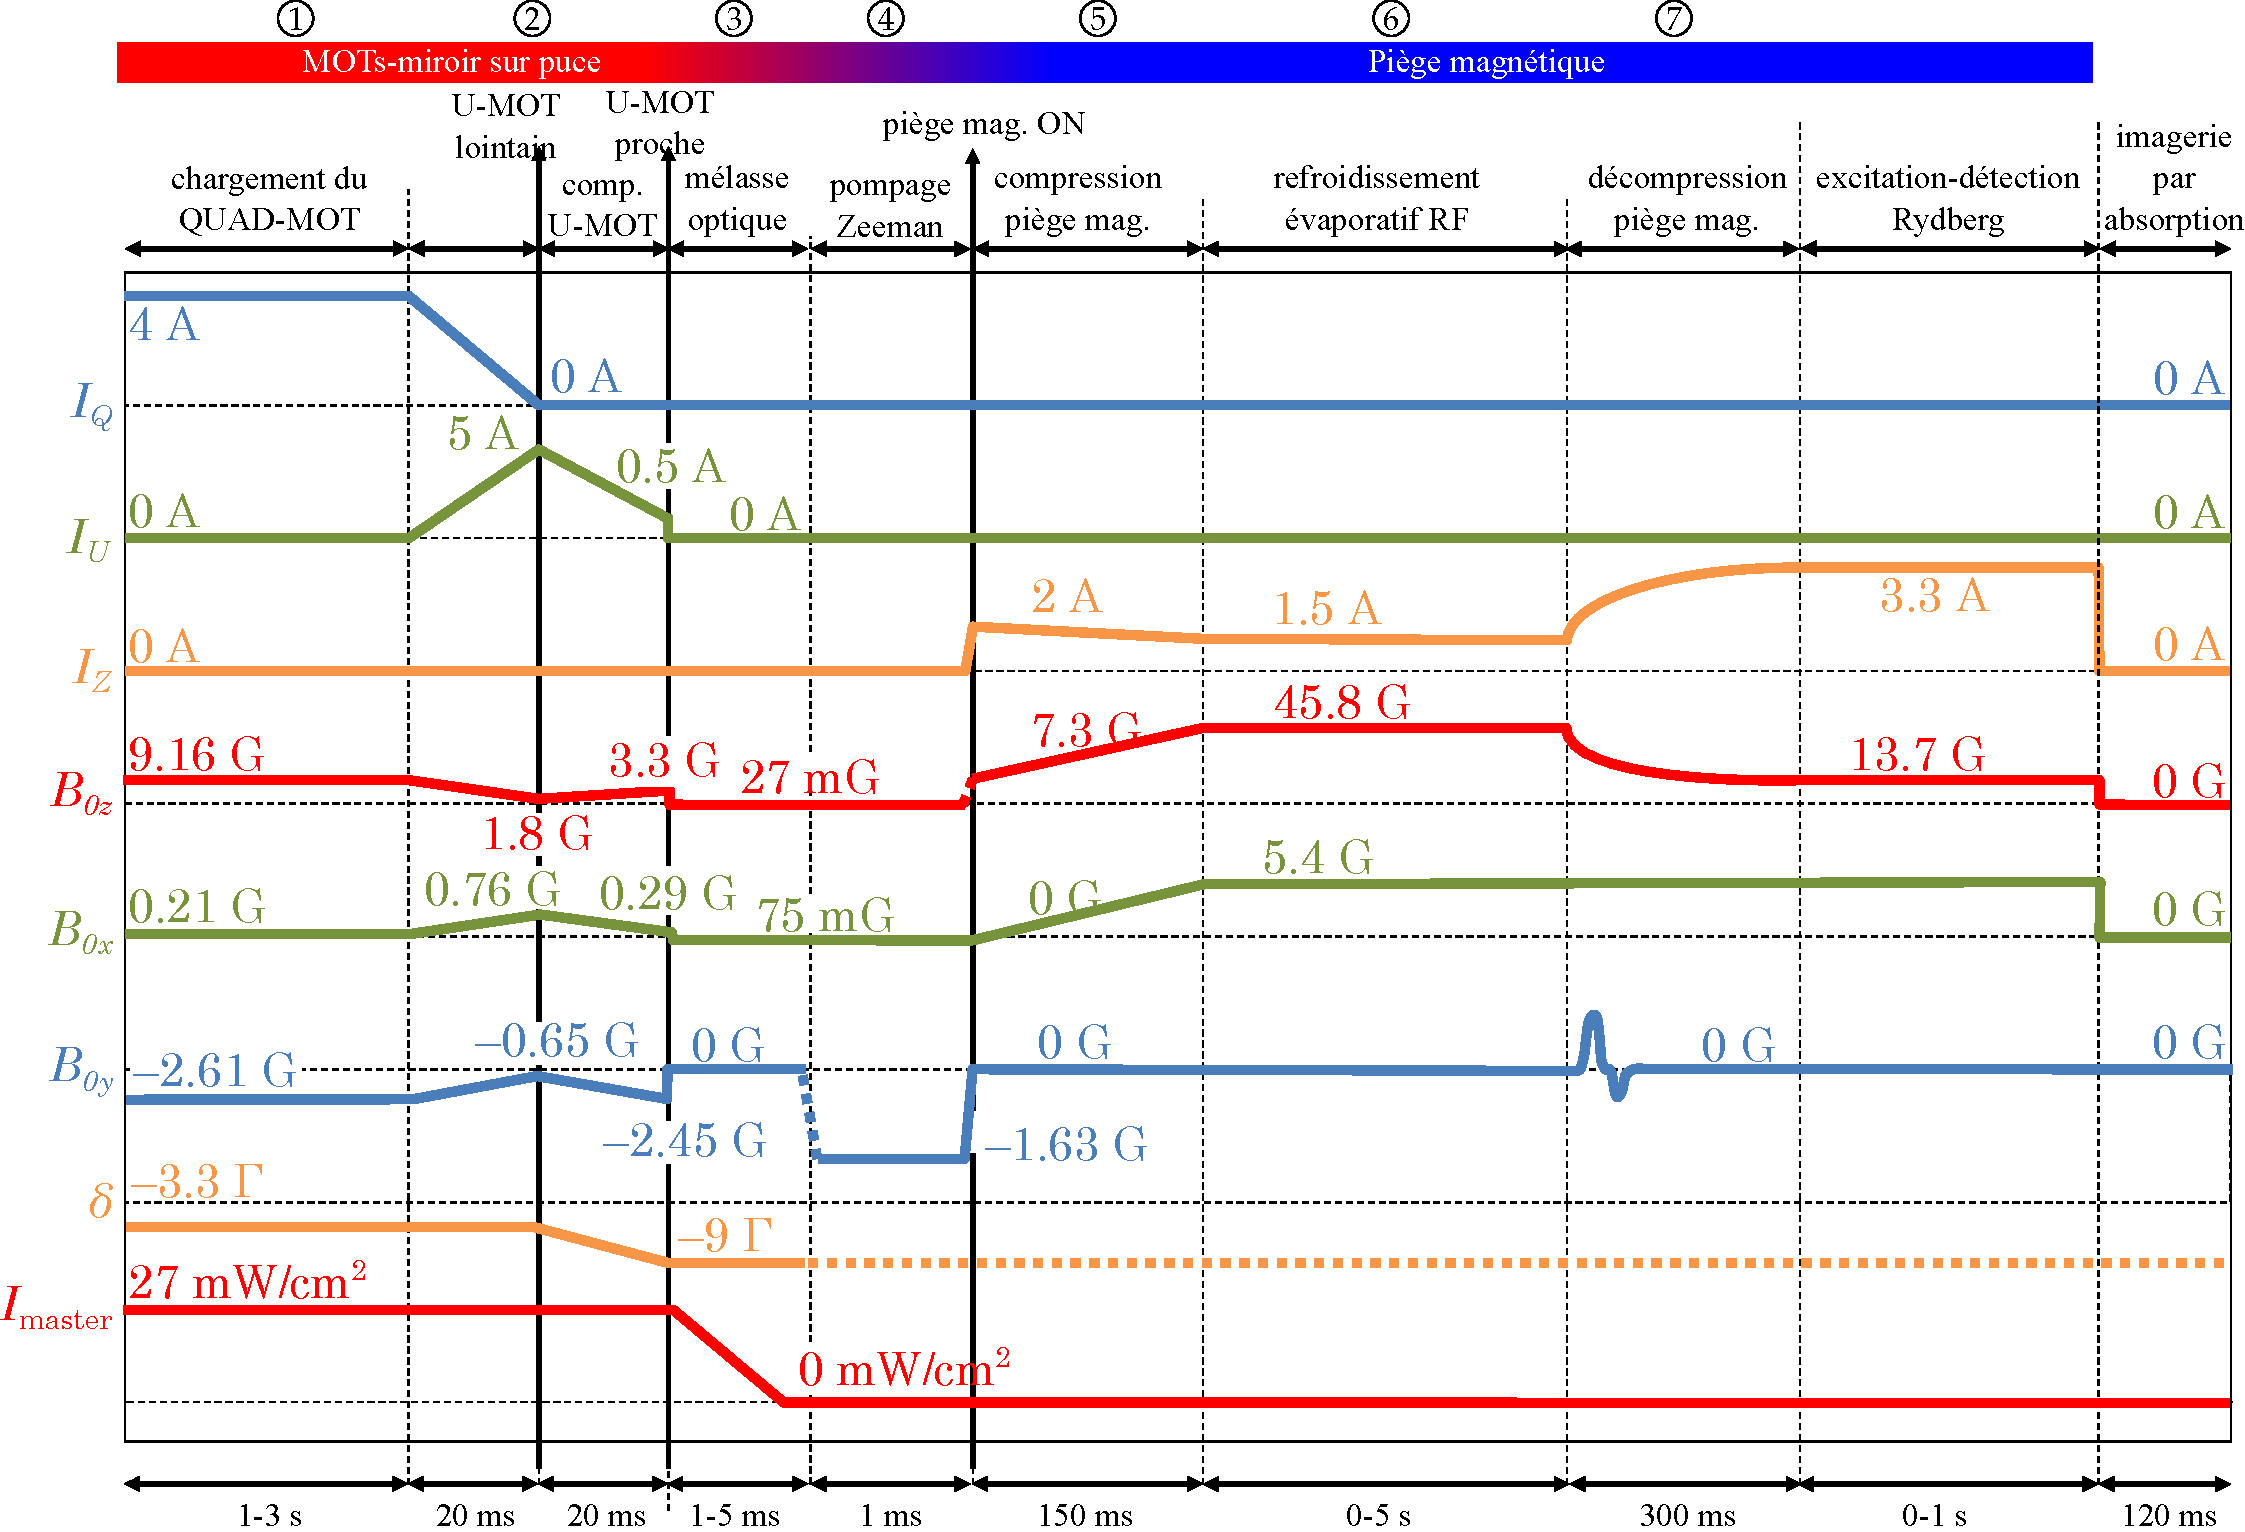
\includegraphics[width=\linewidth]{figures/exp_sequence}
\caption[Séquence expérimentale typique]{Séquence expérimentale typique : la durée et les valeurs des paramètres à chaque étape sont précautionneusement optimisés.
Les étapes de piégeage et de refroidissement sont numérotées de \numrange{1}{7} et discutées dans le texte.
Les étapes ultérieures seront décrites par la suite.
$I_{Q,U,Z}$ sont les courants dans la bobine QUAD, le fil \mcal{U} et le fil \mcal{Z}, en Ampères.
$B_{0~x,y,z}$ sont les champs de biais générés par les bobines dans les directions $x,y,z$, en Gauss.
$\delta$ est le désaccord du laser en unité de la largeur de raie $\Gamma=\SI{6.065}{\MHz}$, et $I_{master}$ son intensité en \si[per-mode=symbol]{\milli\watt \per\squared\cm}.
}
\label{fig:exp_sequence}
\end{sidewaysfigure}
%

\bigskip

		\noindent piégeage magnéto-optique : 2D-MOT, QUAD-MOT, U-MOT \\
		
		\noindent piégeage magnétique de Ioffe Pritchard : principe et potentiel créé par le fil Z (cf. code Mathematica Radia)\\
		
		\noindent refroidissement évaporatif jusqu'au BEC : principe de l'évaporation RF et fils d'évap sur la puce
		
	\subsection{imagerie atomique}
		\noindent optique d'imagerie : schéma optique et caractéristiques des caméras \\
		
		\noindent imagerie par absorption : transition sonde, intensité de saturation \\
		\noindent imagerie par réflexion sur la puce : spécificités de la géométrie et double absoprtion du faisceau sonde \\
		
		\noindent tweaks : absorption no-log et réduction des franges : qu'a-t-on utilisé comme méthodes de traitement pour améliorer notre imagerie $\rightarrow$ un paragraphe sur la réduction de franges et un(ou deux) paragraphe(s) sur l'absorption no-log et sa pertinence dans les mesures de mélasses.
		
	\subsection{nuages typiques}
		\noindent quels MOTs, mélasses et nuages froids obtenus : tailles, températures, nombres d'atomes, distance à la puce.